\documentclass[11pt,a4paper]{article}
\usepackage[margin=23mm]{geometry}
\usepackage[T1]{fontenc}
\usepackage{lmodern,amsmath,amssymb,graphicx,booktabs,microtype}
\usepackage[colorlinks=true,linkcolor=blue,urlcolor=blue,citecolor=blue]{hyperref}
\newcommand{\NodeError}{5.204\times10^{-18}}
\newcommand{\LinearError}{7.568\times10^{-2}}
\newcommand{\FittedError}{1.271\times10^{-17}}
\newcommand{\QuadratureError}{1.110\times10^{-16}}
\newcommand{\FineMms}{6.259\times10^{-6}}
\newcommand{\MaxResidual}{6.426\times10^{-13}}
\newcommand{\MmsOrder}{1.99998}
\newcommand{\LayerRows}{CENTRAL & -0.42857 & 4.353e-01 & 0.07795 \\
UPWIND & 0.00000 & 1.599e-01 & 0.09376 \\
SG & 0.00000 & 5.204e-18 & 0.07568 \\}
\newcommand{\MmsRows}{20 & 1.600e-03 & 7.296e-04 & 1.307e-03 \\
40 & 4.007e-04 & 1.821e-04 & 3.266e-04 \\
80 & 1.001e-04 & 4.551e-05 & 8.162e-05 \\
160 & 2.504e-05 & 1.138e-05 & 2.040e-05 \\
320 & 6.259e-06 & 2.844e-06 & 5.101e-06 \\}

\setlength{\parindent}{0pt}
\setlength{\parskip}{5pt}
\title{LayerLens: exact nodes do not necessarily resolve\newline a stationary boundary layer}
\author{}
\date{}
\begin{document}
\maketitle
\vspace{-13mm}
\begin{abstract}
An exponentially fitted flux can reproduce nodal values of a constant-coefficient
transport problem without resolving its profile under ordinary linear interpolation.
This study makes that distinction measurable in a small, reproducible verification
package. For a global P\'eclet number of 100 and 20 intervals, the fitted scheme
has nodal maximum error $\NodeError$, but its piecewise linear reconstruction has
$L^2$ error $\LinearError$. A homogeneous exponential reconstruction removes that
particular interpolation error; it is not generally exact for a sourced problem.
A separate variable-diffusion, reaction and manufactured-source experiment gives
observed nodal order $\MmsOrder$. Flux residuals, positivity, and field accuracy are
reported separately. These are synthetic mathematical verification results, not
experimental evidence for a physical transport model.
\end{abstract}

\section{Question and model}
The question is whether accurate nodal samples justify describing a coarse
boundary-layer computation as resolved. Exponential fitting is an established
idea; Scharfetter--Gummel extensions include nonlinear diffusion and preservation
of steady states~\cite{bessemoulin}. The contribution here is an original software
experiment and error-reporting workflow, with no claim of a new numerical method.

Consider the stationary conservative equation on $[0,L]$,
\begin{equation}
 J'(x)+r(x)c(x)=f(x),\qquad J=vc-D(x)c',\qquad
 c(0)=c_L,\quad c(L)=c_R. \label{eq:model}
\end{equation}
The drift $v$ is constant, $D>0$, and $r\geq0$. All reported experiments are
nondimensional. The scalar $c$ can represent a transported concentration, but no
material parameters or measurements are fitted. There is no transient term,
nonlinear reaction, coupled flow, or turbulence closure.

\section{Discrete method}
Let $h_i=x_{i+1}-x_i$, $D_i$ be frozen on edge $i$, and
$P_i=vh_i/D_i$. Solving the homogeneous constant-flux edge problem gives
\begin{equation}
 J_i=a_i c_i-b_i c_{i+1},\quad
 a_i=\frac{D_i}{h_i}B(-P_i),\quad b_i=\frac{D_i}{h_i}B(P_i),\quad
 B(z)=\frac{z}{e^z-1},\quad B(0)=1. \label{eq:flux}
\end{equation}
The interior vertex-centered dual volume has width
$w_i=(h_{i-1}+h_i)/2$. Lumped source and reaction integration gives
\begin{equation}
 -a_{i-1}c_{i-1}+(a_i+b_{i-1}+r_iw_i)c_i-b_ic_{i+1}=f_iw_i.
 \label{eq:balance}
\end{equation}
Dirichlet terms move to the right-hand side. Since $B(z)>0$ for finite real $z$
in exact arithmetic and $a_i-b_i=v$, the matrix has nonpositive off-diagonals
and weak row diagonal dominance, with boundary anchoring. Thus the fitted
system is an M-matrix: nonnegative boundary data and source yield nonnegative
nodal values. This statement does not assert an upper bound of one with a
positive source, nor immunity to floating-point conditioning.

\newpage
\section{Implementation and constant-coefficient experiment}
Python evaluates flux coefficients and assembles three matrix bands; SciPy's
banded solver~\cite{scipy} supplies the compiled direct linear algebra. Assembly,
storage, and tridiagonal solution scale linearly in the number of nodes. A separate
C++ wrapper would add packaging complexity without a demonstrated need here.
For $q=|z|$, evaluation uses $B(q)=q e^{-q}/(1-e^{-q})$ and
$B(-q)=B(q)+q$, with a local Taylor expansion near zero. This avoids positive
exponent overflow. Inputs are checked for shape, finiteness, ordered nodes,
positive diffusion and nonnegative reaction. Returned arrays are read-only
snapshots; invalid reconstruction queries are rejected rather than extrapolated.

Two diagnostic comparators use the same balance equation: central differencing
sets $a=D/h+v/2$, $b=D/h-v/2$; upwind sets
$a=D/h+\max(v,0)$, $b=D/h+\max(-v,0)$. The central off-diagonal sign condition
fails when $|P|>2$. No limiter or clipping conceals that failure.

The first experiment uses $L=1$, $v=1$, $D=0.01$, $r=f=0$, and $(c_L,c_R)=(0,1)$.
Its exact solution is $c(x)=(e^{100x}-1)/(e^{100}-1)$, evaluated in a scaled
form. Uniform grids contain $N=20,40,80,160,320$ intervals.
The independently reported errors are
\begin{equation}
 E_{\rm node}=\max_i|c_i-c(x_i)|,\qquad
 E_{\rm field}=\left[\int_0^1|\mathcal R c_h-c(x)|^2\,dx\right]^{1/2}.
\end{equation}
Here $\mathcal R$ is explicitly linear or homogeneous exponential interpolation.
The latter uses the normalized edge profile
$\theta(t)=(e^{P_it}-1)/(e^{P_i}-1)$, $t=(x-x_i)/h_i$.
Per-edge 32-point Gauss--Legendre integration computes field norms. Increasing to
64 points changes the coarse fitted linear-field norm by $\QuadratureError$.

\begin{figure}[h]
\centering
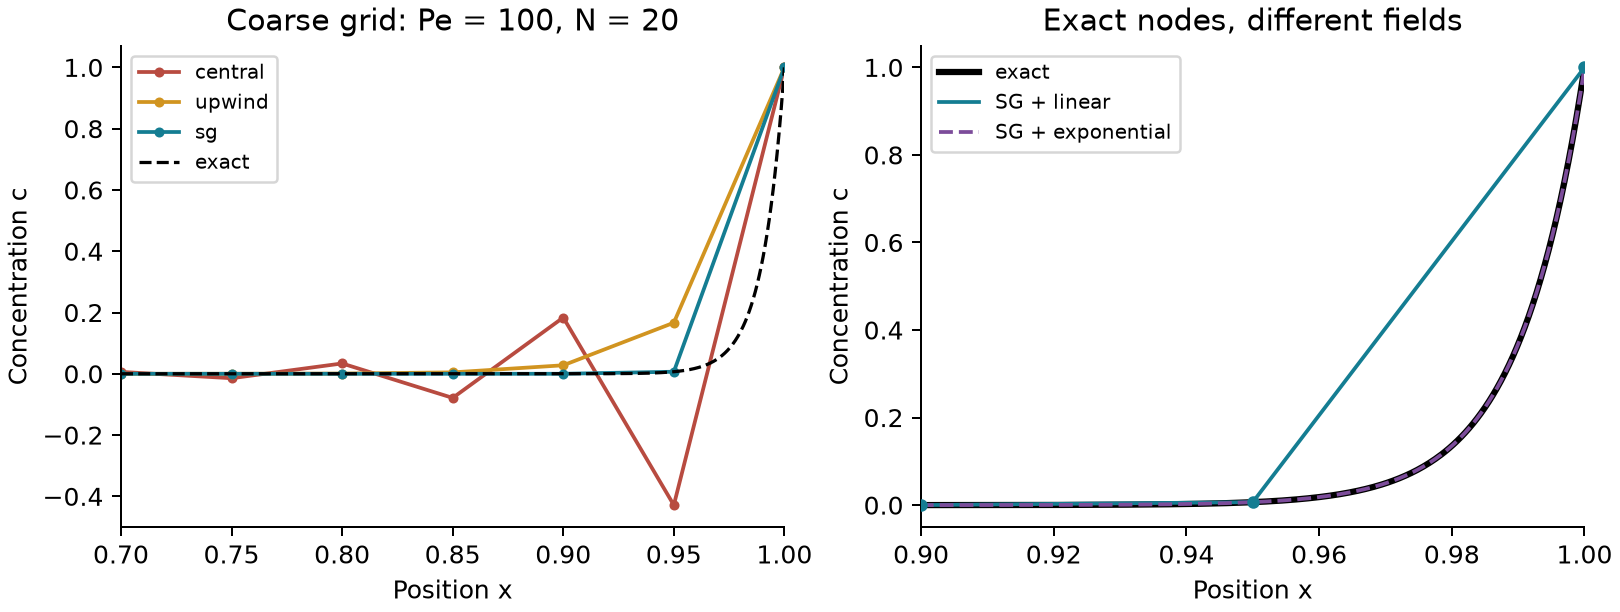
\includegraphics[width=\linewidth]{../examples/results/boundary_layer.png}
\caption{Original computed profiles. Left: central oscillation and upwind
smearing. Right: identical fitted nodal values support two different fields.}
\end{figure}
\vspace{-3mm}
\begin{table}[h]
\centering
\caption{Recorded coarse-grid results ($N=20$, edge $P=5$).}
\begin{tabular}{lrrr}\toprule
Scheme & Minimum $c_i$ & $E_{\rm node}$ & Linear $E_{\rm field}$\\\midrule
\LayerRows
\bottomrule\end{tabular}
\end{table}

\newpage
\section{Manufactured solution and measured convergence}
Constant-coefficient nodal exactness is a narrow property. To test source,
reaction, and variable-diffusion assembly independently, a manufactured
solution~\cite{salari} is prescribed:
\begin{equation}
 c_*(x)=1+x+\sin(\pi x),\quad v=2,\quad D(x)=1+x,\quad r=0.7,
 \qquad 0\leq x\leq1.
\end{equation}
With boundary values $(1,2)$, the source is derived directly from
Eq.~\eqref{eq:model}: $f=c_*'-(1+x)c_*''+0.7c_*$.
The diffusivity is sampled at edge midpoints; source and reaction use interior
nodes and the weights in Eq.~\eqref{eq:balance}. The same five grids are used.
Table~\ref{tab:mms} and Fig.~\ref{fig:convergence} contain actual recorded outputs.

\begin{figure}[h]
\centering
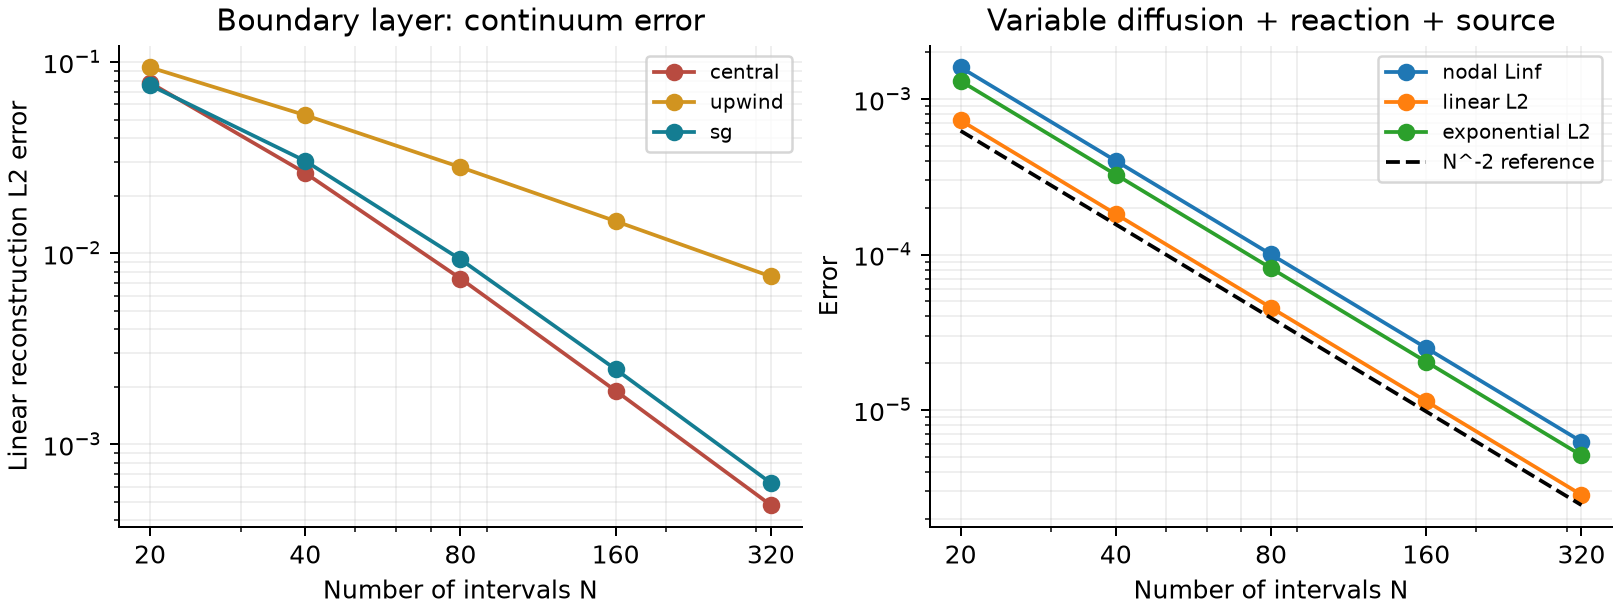
\includegraphics[width=\linewidth]{../examples/results/convergence.png}
\caption{Left: continuum errors with linear reconstruction for the boundary
layer. Right: errors for the manufactured problem. The reference line indicates
slope only; it is not an error bound.}\label{fig:convergence}
\end{figure}
\vspace{-3mm}
\begin{table}[h]
\centering
\caption{Manufactured problem, fitted scheme. All errors are absolute.}
\label{tab:mms}
\begin{tabular}{rrrr}\toprule
$N$ & $E_{\rm node}$ & Linear $E_{\rm field}$ & Exponential $E_{\rm field}$\\\midrule
\MmsRows
\bottomrule\end{tabular}
\end{table}

The final nodal error is $\FineMms$; the last refinement gives
$\log_2(E_{160}/E_{320})=\MmsOrder$. The maximum absolute dual-cell balance
residual across these grids is $\MaxResidual$. A residual is a discrete equation
defect, not a discretization-error estimator. Summing it gives the net flux plus
lumped reaction-minus-source defect over the interior dual cells only; the
Dirichlet endpoint half-cells are not separate conservation equations.

\section{Discussion: what is actually accurate?}
For the homogeneous problem, fitting captures the exact relation between two
nodal values, even when a cell is wider than the layer. The exponential
reconstruction then attains $L^2$ error $\FittedError$ on the coarse grid.
Linear interpolation instead spreads a steep change over an entire cell.
Both reconstructions share the same algebraic residual and the same nodes, so
neither diagnostic can identify the between-node discrepancy by itself.

With a source and variable diffusion, exponential reconstruction is not exact;
here its field error exceeds that of linear interpolation. Both converge with
refinement. A reported continuum norm must therefore name its reconstruction.

\newpage
\section{Verification scope and reproducibility}
Tests cover analytic solutions, signed drift, positive sources, graded meshes,
manufactured convergence, central oscillations, and invalid inputs. Profile tests
span global P\'eclet values from $-1000$ to $1000$; Bernoulli checks reach
$\pm10000$. These finite tests are not an exhaustive certification.

Install with \texttt{python -m pip install -e ".[dev]"}; run tests with
\texttt{python -m pytest -q}. Run \texttt{layerlens demo} for tables, metrics,
figures and dependency versions. \texttt{python} \path{scripts/check_samples.py}
reproduces the archived results in a separate directory.
Numeric checks allow relative differences of $5\times10^{-7}$
and absolute differences of $2\times10^{-12}$, with a $2\times10^{-10}$ absolute
tolerance for roundoff-sensitive residual and balance metrics. Image byte
identity is not required across Matplotlib versions.

Tables and numerical macros come from the recorded JSON. The paper build checks
references, layout, page count and input hashes. CI reproduces results, tests the
installed wheel, and archives the compiled paper and rendered pages.
The README records executed checks. No course documents or private data are
distributed.

\section{Limitations and physical interpretation}
The library supports only stationary one-dimensional scalar transport with
constant drift and Dirichlet data. Midpoint diffusion freezing and lumped
source/reaction integration introduce approximation error. The measured
second-order result applies to one smooth solution on uniform grids, not
automatically to abrupt mesh grading or coefficient jumps.

Large positive Bernoulli arguments underflow to zero, creating an effectively
one-sided floating-point limit. Mesh grading and coefficient contrast may impair
conditioning. There is no certified condition estimator or a posteriori error
bound. Small absolute residuals do not imply relative accuracy for exponentially
small fluxes. Central differences are an intentionally non-monotone comparator.

These experiments probe discrete correctness and continuum approximation, not
physical validity. The latter requires an application-specific model and
measurements. No real device, material or flow is validated here.

\section{Conclusion}
Nodal exactness can coexist with reconstruction error. Verification must name
the reconstruction and distinguish conservation from accuracy. Sign, balance,
and second-order convergence checks support this implementation for the tested
problems; they do not establish exactness for general transport.

\begin{thebibliography}{9}\small
\bibitem{bessemoulin} M. Bessemoulin-Chatard. A finite volume scheme for
convection-diffusion equations with nonlinear diffusion derived from the
Scharfetter--Gummel scheme. arXiv:1011.2299v2, 2012.
\href{https://arxiv.org/abs/1011.2299}{arXiv:1011.2299}.
\bibitem{salari} K. Salari and P. Knupp. Code Verification by the Method of
Manufactured Solutions. Sandia report SAND2000-1444, 2000.
\href{https://doi.org/10.2172/759450}{doi:10.2172/759450}.
\bibitem{scipy} SciPy developers. \texttt{scipy.linalg.solve\_banded}, API reference.
\href{https://docs.scipy.org/doc/scipy/reference/generated/scipy.linalg.solve_banded.html}{Official documentation}, accessed 1 October 2026.
\end{thebibliography}
\end{document}
